
%% This style is provided for the ICSE 2015 main conference,
%% ICSE 2015 co-located events, and ICSE 2015 workshops.

%% bare_conf_ICSE15.tex
%% V1.4
%% 2014/05/22


%% This is a skeleton file demonstrating the use of IEEEtran.cls
%% (requires IEEEtran.cls version 1.7 or later) with an IEEE conference paper.
%%
%% Support sites:
%% http://www.michaelshell.org/tex/ieeetran/
%% http://www.ctan.org/tex-archive/macros/latex/contrib/IEEEtran/
%% and
%% http://www.ieee.org/

%%*************************************************************************
%% Legal Notice:
%% This code is offered as-is without any warranty either expressed or
%% implied; without even the implied warranty of MERCHANTABILITY or
%% FITNESS FOR A PARTICULAR PURPOSE!
%% User assumes all risk.
%% In no event shall IEEE or any contributor to this code be liable for
%% any damages or losses, including, but not limited to, incidental,
%% consequential, or any other damages, resulting from the use or misuse
%% of any information contained here.
%%
%% All comments are the opinions of their respective authors and are not
%% necessarily endorsed by the IEEE.
%%
%% This work is distributed under the LaTeX Project Public License (LPPL)
%% ( http://www.latex-project.org/ ) version 1.3, and may be freely used,
%% distributed and modified. A copy of the LPPL, version 1.3, is included
%% in the base LaTeX documentation of all distributions of LaTeX released
%% 2003/12/01 or later.
%% Retain all contribution notices and credits.
%% ** Modified files should be clearly indicated as such, including  **
%% ** renaming them and changing author support contact information. **
%%
%% File list of work: IEEEtran.cls, IEEEtran_HOWTO.pdf, bare_adv.tex,
%%                    bare_conf.tex, bare_jrnl.tex, bare_jrnl_compsoc.tex
%%*************************************************************************

% *** Authors should verify (and, if needed, correct) their LaTeX system  ***
% *** with the testflow diagnostic prior to trusting their LaTeX platform ***
% *** with production work. IEEE's font choices can trigger bugs that do  ***
% *** not appear when using other class files.                            ***
% The testflow support page is at:
% http://www.michaelshell.org/tex/testflow/



% Note that the a4paper option is mainly intended so that authors in
% countries using A4 can easily print to A4 and see how their papers will
% look in print - the typesetting of the document will not typically be
% affected with changes in paper size (but the bottom and side margins will).
% Use the testflow package mentioned above to verify correct handling of
% both paper sizes by the user's LaTeX system.
%
% Also note that the "draftcls" or "draftclsnofoot", not "draft", option
% should be used if it is desired that the figures are to be displayed in
% draft mode.
%
\documentclass[conference]{IEEEtran}
%
% If IEEEtran.cls has not been installed into the LaTeX system files,
% manually specify the path to it like:
% \documentclass[conference]{../sty/IEEEtran}





% Some very useful LaTeX packages include:
% (uncomment the ones you want to load)


% *** MISC UTILITY PACKAGES ***
%
%\usepackage{ifpdf}
% Heiko Oberdiek's ifpdf.sty is very useful if you need conditional
% compilation based on whether the output is pdf or dvi.
% usage:
% \ifpdf
%   % pdf code
% \else
%   % dvi code
% \fi
% The latest version of ifpdf.sty can be obtained from:
% http://www.ctan.org/tex-archive/macros/latex/contrib/oberdiek/
% Also, note that IEEEtran.cls V1.7 and later provides a builtin
% \ifCLASSINFOpdf conditional that works the same way.
% When switching from latex to pdflatex and vice-versa, the compiler may
% have to be run twice to clear warning/error messages.






% *** CITATION PACKAGES ***
%
%\usepackage{cite}
% cite.sty was written by Donald Arseneau
% V1.6 and later of IEEEtran pre-defines the format of the cite.sty package
% \cite{} output to follow that of IEEE. Loading the cite package will
% result in citation numbers being automatically sorted and properly
% "compressed/ranged". e.g., [1], [9], [2], [7], [5], [6] without using
% cite.sty will become [1], [2], [5]--[7], [9] using cite.sty. cite.sty's
% \cite will automatically add leading space, if needed. Use cite.sty's
% noadjust option (cite.sty V3.8 and later) if you want to turn this off.
% cite.sty is already installed on most LaTeX systems. Be sure and use
% version 4.0 (2003-05-27) and later if using hyperref.sty. cite.sty does
% not currently provide for hyperlinked citations.
% The latest version can be obtained at:
% http://www.ctan.org/tex-archive/macros/latex/contrib/cite/
% The documentation is contained in the cite.sty file itself.






% *** GRAPHICS RELATED PACKAGES ***
%
\ifCLASSINFOpdf
  % \usepackage[pdftex]{graphicx}
  % declare the path(s) where your graphic files are
  % \graphicspath{{../pdf/}{../jpeg/}}
  % and their extensions so you won't have to specify these with
  % every instance of \includegraphics
  % \DeclareGraphicsExtensions{.pdf,.jpeg,.png}
\else
  % or other class option (dvipsone, dvipdf, if not using dvips). graphicx
  % will default to the driver specified in the system graphics.cfg if no
  % driver is specified.
  % \usepackage[dvips]{graphicx}
  % declare the path(s) where your graphic files are
  % \graphicspath{{../eps/}}
  % and their extensions so you won't have to specify these with
  % every instance of \includegraphics
  % \DeclareGraphicsExtensions{.eps}
\fi
% graphicx was written by David Carlisle and Sebastian Rahtz. It is
% required if you want graphics, photos, etc. graphicx.sty is already
% installed on most LaTeX systems. The latest version and documentation can
% be obtained at:
% http://www.ctan.org/tex-archive/macros/latex/required/graphics/
% Another good source of documentation is "Using Imported Graphics in
% LaTeX2e" by Keith Reckdahl which can be found as epslatex.ps or
% epslatex.pdf at: http://www.ctan.org/tex-archive/info/
%
% latex, and pdflatex in dvi mode, support graphics in encapsulated
% postscript (.eps) format. pdflatex in pdf mode supports graphics
% in .pdf, .jpeg, .png and .mps (metapost) formats. Users should ensure
% that all non-photo figures use a vector format (.eps, .pdf, .mps) and
% not a bitmapped formats (.jpeg, .png). IEEE frowns on bitmapped formats
% which can result in "jaggedy"/blurry rendering of lines and letters as
% well as large increases in file sizes.
%
% You can find documentation about the pdfTeX application at:
% http://www.tug.org/applications/pdftex





% *** MATH PACKAGES ***
%
%\usepackage[cmex10]{amsmath}
% A popular package from the American Mathematical Society that provides
% many useful and powerful commands for dealing with mathematics. If using
% it, be sure to load this package with the cmex10 option to ensure that
% only type 1 fonts will utilized at all point sizes. Without this option,
% it is possible that some math symbols, particularly those within
% footnotes, will be rendered in bitmap form which will result in a
% document that can not be IEEE Xplore compliant!
%
% Also, note that the amsmath package sets \interdisplaylinepenalty to 10000
% thus preventing page breaks from occurring within multiline equations. Use:
%\interdisplaylinepenalty=2500
% after loading amsmath to restore such page breaks as IEEEtran.cls normally
% does. amsmath.sty is already installed on most LaTeX systems. The latest
% version and documentation can be obtained at:
% http://www.ctan.org/tex-archive/macros/latex/required/amslatex/math/





% *** SPECIALIZED LIST PACKAGES ***
%
%\usepackage{algorithmic}
% algorithmic.sty was written by Peter Williams and Rogerio Brito.
% This package provides an algorithmic environment fo describing algorithms.
% You can use the algorithmic environment in-text or within a figure
% environment to provide for a floating algorithm. Do NOT use the algorithm
% floating environment provided by algorithm.sty (by the same authors) or
% algorithm2e.sty (by Christophe Fiorio) as IEEE does not use dedicated
% algorithm float types and packages that provide these will not provide
% correct IEEE style captions. The latest version and documentation of
% algorithmic.sty can be obtained at:
% http://www.ctan.org/tex-archive/macros/latex/contrib/algorithms/
% There is also a support site at:
% http://algorithms.berlios.de/index.html
% Also of interest may be the (relatively newer and more customizable)
% algorithmicx.sty package by Szasz Janos:
% http://www.ctan.org/tex-archive/macros/latex/contrib/algorithmicx/




% *** ALIGNMENT PACKAGES ***
%
%\usepackage{array}
% Frank Mittelbach's and David Carlisle's array.sty patches and improves
% the standard LaTeX2e array and tabular environments to provide better
% appearance and additional user controls. As the default LaTeX2e table
% generation code is lacking to the point of almost being broken with
% respect to the quality of the end results, all users are strongly
% advised to use an enhanced (at the very least that provided by array.sty)
% set of table tools. array.sty is already installed on most systems. The
% latest version and documentation can be obtained at:
% http://www.ctan.org/tex-archive/macros/latex/required/tools/


%\usepackage{mdwmath}
%\usepackage{mdwtab}
% Also highly recommended is Mark Wooding's extremely powerful MDW tools,
% especially mdwmath.sty and mdwtab.sty which are used to format equations
% and tables, respectively. The MDWtools set is already installed on most
% LaTeX systems. The lastest version and documentation is available at:
% http://www.ctan.org/tex-archive/macros/latex/contrib/mdwtools/


% IEEEtran contains the IEEEeqnarray family of commands that can be used to
% generate multiline equations as well as matrices, tables, etc., of high
% quality.


%\usepackage{eqparbox}
% Also of notable interest is Scott Pakin's eqparbox package for creating
% (automatically sized) equal width boxes - aka "natural width parboxes".
% Available at:
% http://www.ctan.org/tex-archive/macros/latex/contrib/eqparbox/





% *** SUBFIGURE PACKAGES ***
%\usepackage[tight,footnotesize]{subfigure}
% subfigure.sty was written by Steven Douglas Cochran. This package makes it
% easy to put subfigures in your figures. e.g., "Figure 1a and 1b". For IEEE
% work, it is a good idea to load it with the tight package option to reduce
% the amount of white space around the subfigures. subfigure.sty is already
% installed on most LaTeX systems. The latest version and documentation can
% be obtained at:
% http://www.ctan.org/tex-archive/obsolete/macros/latex/contrib/subfigure/
% subfigure.sty has been superceeded by subfig.sty.



%\usepackage[caption=false]{caption}
%\usepackage[font=footnotesize]{subfig}
% subfig.sty, also written by Steven Douglas Cochran, is the modern
% replacement for subfigure.sty. However, subfig.sty requires and
% automatically loads Axel Sommerfeldt's caption.sty which will override
% IEEEtran.cls handling of captions and this will result in nonIEEE style
% figure/table captions. To prevent this problem, be sure and preload
% caption.sty with its "caption=false" package option. This is will preserve
% IEEEtran.cls handing of captions. Version 1.3 (2005/06/28) and later
% (recommended due to many improvements over 1.2) of subfig.sty supports
% the caption=false option directly:
%\usepackage[caption=false,font=footnotesize]{subfig}
%
% The latest version and documentation can be obtained at:
% http://www.ctan.org/tex-archive/macros/latex/contrib/subfig/
% The latest version and documentation of caption.sty can be obtained at:
% http://www.ctan.org/tex-archive/macros/latex/contrib/caption/




% *** FLOAT PACKAGES ***
%
%\usepackage{fixltx2e}
% fixltx2e, the successor to the earlier fix2col.sty, was written by
% Frank Mittelbach and David Carlisle. This package corrects a few problems
% in the LaTeX2e kernel, the most notable of which is that in current
% LaTeX2e releases, the ordering of single and double column floats is not
% guaranteed to be preserved. Thus, an unpatched LaTeX2e can allow a
% single column figure to be placed prior to an earlier double column
% figure. The latest version and documentation can be found at:
% http://www.ctan.org/tex-archive/macros/latex/base/



%\usepackage{stfloats}
% stfloats.sty was written by Sigitas Tolusis. This package gives LaTeX2e
% the ability to do double column floats at the bottom of the page as well
% as the top. (e.g., "\begin{figure*}[!b]" is not normally possible in
% LaTeX2e). It also provides a command:
%\fnbelowfloat
% to enable the placement of footnotes below bottom floats (the standard
% LaTeX2e kernel puts them above bottom floats). This is an invasive package
% which rewrites many portions of the LaTeX2e float routines. It may not work
% with other packages that modify the LaTeX2e float routines. The latest
% version and documentation can be obtained at:
% http://www.ctan.org/tex-archive/macros/latex/contrib/sttools/
% Documentation is contained in the stfloats.sty comments as well as in the
% presfull.pdf file. Do not use the stfloats baselinefloat ability as IEEE
% does not allow \baselineskip to stretch. Authors submitting work to the
% IEEE should note that IEEE rarely uses double column equations and
% that authors should try to avoid such use. Do not be tempted to use the
% cuted.sty or midfloat.sty packages (also by Sigitas Tolusis) as IEEE does
% not format its papers in such ways.





% *** PDF, URL AND HYPERLINK PACKAGES ***
%
%\usepackage{url}
% url.sty was written by Donald Arseneau. It provides better support for
% handling and breaking URLs. url.sty is already installed on most LaTeX
% systems. The latest version can be obtained at:
% http://www.ctan.org/tex-archive/macros/latex/contrib/misc/
% Read the url.sty source comments for usage information. Basically,
% \url{my_url_here}.





% *** Do not adjust lengths that control margins, column widths, etc. ***
% *** Do not use packages that alter fonts (such as pslatex).         ***
% There should be no need to do such things with IEEEtran.cls V1.6 and later.
% (Unless specifically asked to do so by the journal or conference you plan
% to submit to, of course. )


% correct bad hyphenation here
\hyphenation{op-tical net-works semi-conduc-tor}

\usepackage{graphicx}

\begin{document}
%
% paper title
% can use linebreaks \\ within to get better formatting as desired
\title{Why the vast majority of StackOverflow only posts one question}


% author names and affiliations
% use a multiple column layout for up to three different
% affiliations
\author{\IEEEauthorblockN{Rogier Slag}
\IEEEauthorblockA{Delft University of Technology\\
Delft, the Netherlands\\
1507761\\
rogier.slag@gmail.com
}
\and
\IEEEauthorblockN{Mike de Waard}
\IEEEauthorblockA{Delft University of Technology\\
Delft, the Netherlands\\
4081064\\
mikedewaard@gmail.com}}


% conference papers do not typically use \thanks and this command
% is locked out in conference mode. If really needed, such as for
% the acknowledgment of grants, issue a \IEEEoverridecommandlockouts
% after \documentclass

% for over three affiliations, or if they all won't fit within the width
% of the page, use this alternative format:
% 
%\author{\IEEEauthorblockN{Michael Shell\IEEEauthorrefmark{1},
%Homer Simpson\IEEEauthorrefmark{2},
%James Kirk\IEEEauthorrefmark{3}, 
%Montgomery Scott\IEEEauthorrefmark{3} and
%Eldon Tyrell\IEEEauthorrefmark{4}}
%\IEEEauthorblockA{\IEEEauthorrefmark{1}School of Electrical and Computer Engineering\\
%Georgia Institute of Technology,
%Atlanta, Georgia 30332--0250\\ Email: see http://www.michaelshell.org/contact.html}
%\IEEEauthorblockA{\IEEEauthorrefmark{2}Twentieth Century Fox, Springfield, USA\\
%Email: homer@thesimpsons.com}
%\IEEEauthorblockA{\IEEEauthorrefmark{3}Starfleet Academy, San Francisco, California 96678-2391\\
%Telephone: (800) 555--1212, Fax: (888) 555--1212}
%\IEEEauthorblockA{\IEEEauthorrefmark{4}Tyrell Inc., 123 Replicant Street, Los Angeles, California 90210--4321}}




% use for special paper notices
%\IEEEspecialpapernotice{(Invited Paper)}




% make the title area
\maketitle


\begin{abstract}

%\boldmath

While StackOverflow is a very well-known platform in the programming industry, the Q\&A section is only effectively filled with content by a low number of users. Within that user group, around $75\%$ only makes one contribution to the platform in total. Since the platform is that popular, how come the number of participants is that low?
\\
\\
This paper defines a group called the \textit{one-day flies} and tries to find reasons these users do not continue to contribute to the platform. By enabling users to become more active, the community itself could grow even further and continue to deliver answers to programmers all over the world.\\
\\
To do this, we analyze a public StackOverflow database dump  for several assumptions. These are  compared between the one-day flies and the regular user group, in order to find statistical differences between these groups on certain level. 

\end{abstract}

\IEEEpeerreviewmaketitle



\section{Introduction}

StackOverflow is a Q\&A community on the Internet, which is managed by the StackExchange platform. It focuses primarily on programming related questions, and is the biggest Q\&A community on that specific topic.
\\
\\
StackOverflow has been gaining popularity during the last few years \cite{SOPopularity}, and lots of research has been done on the data corpus of StackOverflow, such as \cite{SOResearch1}, \cite{SOResearch2} and \cite{SOResearch3}. These and many other research papers on StackOverflow are about the users personalities \cite{buildingrep}, their field of expertise and on how these users contribute \cite{repsystem}, but not so much research has gone into how the underlying structure of the StackOverflow community. With underlying structure we mean, for example the distribution of posts among users, the distribution of reputation among users, and so on.
\\
\\
This is why we started with some exploratory data analysis on the StackOverflow Data, which revealed that over $75\%$ of the users posted only twice or even less during their whole registration period. Given this high amount of  \textit{one-day flies} we analyzed what happens to the content that these people contribute to the system. The initial idea was that most of these single-posts could be either marked as duplicate, very specific to a certain domain / programming language and do not get answered, or reveal a flaw in the documentation of an API. To elaborate a bit further on the flaw in API Documentation, a one-day fly can ask a question regarding how to use a specific API but not have any further questions for StackOverflow as he/she is an experienced developer. However during this research interesting findings regarding these initial beliefs emerged.


\section{Related work}

By being one of the largest, and most well-known Q\&A platform regarding programming related questions, StackOverflow is an interesting community for researchers. Additionally StackOverflow actively releases parts of its database to the public, which proved to be of an extreme value for researchers. Therefore, it comes as no surprise StackOverflow has attracted a significant amount of researchers in the areas of software engineering,
 and social studies.
\\
\\
Several aspects of StackOverflow have already been investigated, such as how to build reputation \cite{buildingrep}, and how the reputation system encourages users to participate \cite{repsystem}. These works gave us insight in how the reputation system works and how this affects the user base. Other researchers \cite{correa2014chaff}. investigated the deletion of questions on StackOverflow, which we used to verify some of our research questions. 

A group of researchers from Canada \cite{PersonalityTraits} did work on the personality traits of StackOverflow users, which we used as base for the sentimental analysis for post and answers.

And finally related work was done in \cite{sparrowsandowls}, where researchers looked specifically at the group of experts. Our work complements this work such that we look at the group that was left out in this research.
\\



\section{Exploratory Data Analysis}

% How is the stackoverflow data structured, how are the distributions of entities
For this analysis, the StackOverflow data as provided by the 2014 MSR Challenge was used. This data was then preprocessed and saved to a MS-SQL server. This allowed for rapid processing, due to which large parts of the analysis could be done on the entire data set.
\\
\\
After this preprocessing step was completed an exploratory analysis was done on the data set. Since StackOverflow is a regular Q\&A website, focused on programming languages, there was a suspicion it would adhere to general community dynamics specifics. An indicator of this would be a large number of inactive users, a small set of users which are more active, and a very small set of very active users.
\\
\\
To test this, clustering of several user groups was required. Even though  this can be done using several aspects, the number of posts is for most communities applicable, as this is a direct measure for contributions to the community. Moreover StackOverflow has a special reputation system, which gamifies the platform. The reputation is acquired by users through the system and reflects how the contributions of people are received by the community. Using the reputation points earned by the users, they can be classified into several groups. Based  on general community dynamics, a clustering in three groups seemed appropriate, as this would result in inactive (or one-day flies), active and very active user groups.
\\
\\
In the dataset we got from StackOverflow on september 26th in 2014, a total of 2.063.174 users had a reputation of one, whilst the total amount of users of StackOverflow is 3.473.095.This causes the median to  equal to one, whereas the third quartile is just $13$. Compared to the maximum value of $709.269$ it is safe to conclude that a lot of users do not actively participate in the community, either by asking questions or proposing answers.
\\
\\
This can also be seen in the analysis of the number of posts a user made. $75\%$ of the people has made a maximum of two posts. Again here the maximum is shifted towards the other end; the user with the most posts has acquired $30.043$ posts on the website. It therefore seems a large majority of the users has no need nor wish to participate more in the community.
\\
\\
When the clustering into three groups is completed using k-means theory (see figure \ref{kmeans_clustering}), three clusters are obtained, based on the reputation they achieved. The group of what we refer to as one-day-flies is the largest, with a total of $3.469.897$ users. The medium active user group is significantly smaller and only contains $3.012$ users with an average reputation of $38.000$. The group with the most reputation is by far the smallest, and only contains $186$ users. The average reputation of this group is then very high (almost $200.000$).
\\
\\
When correlated with the number of posts or comments, it appears there is a linear relation between those on one hand and reputation on the other hand. The center groups of the clustering almost form one straight line when plotted.

\begin{figure}[h]
 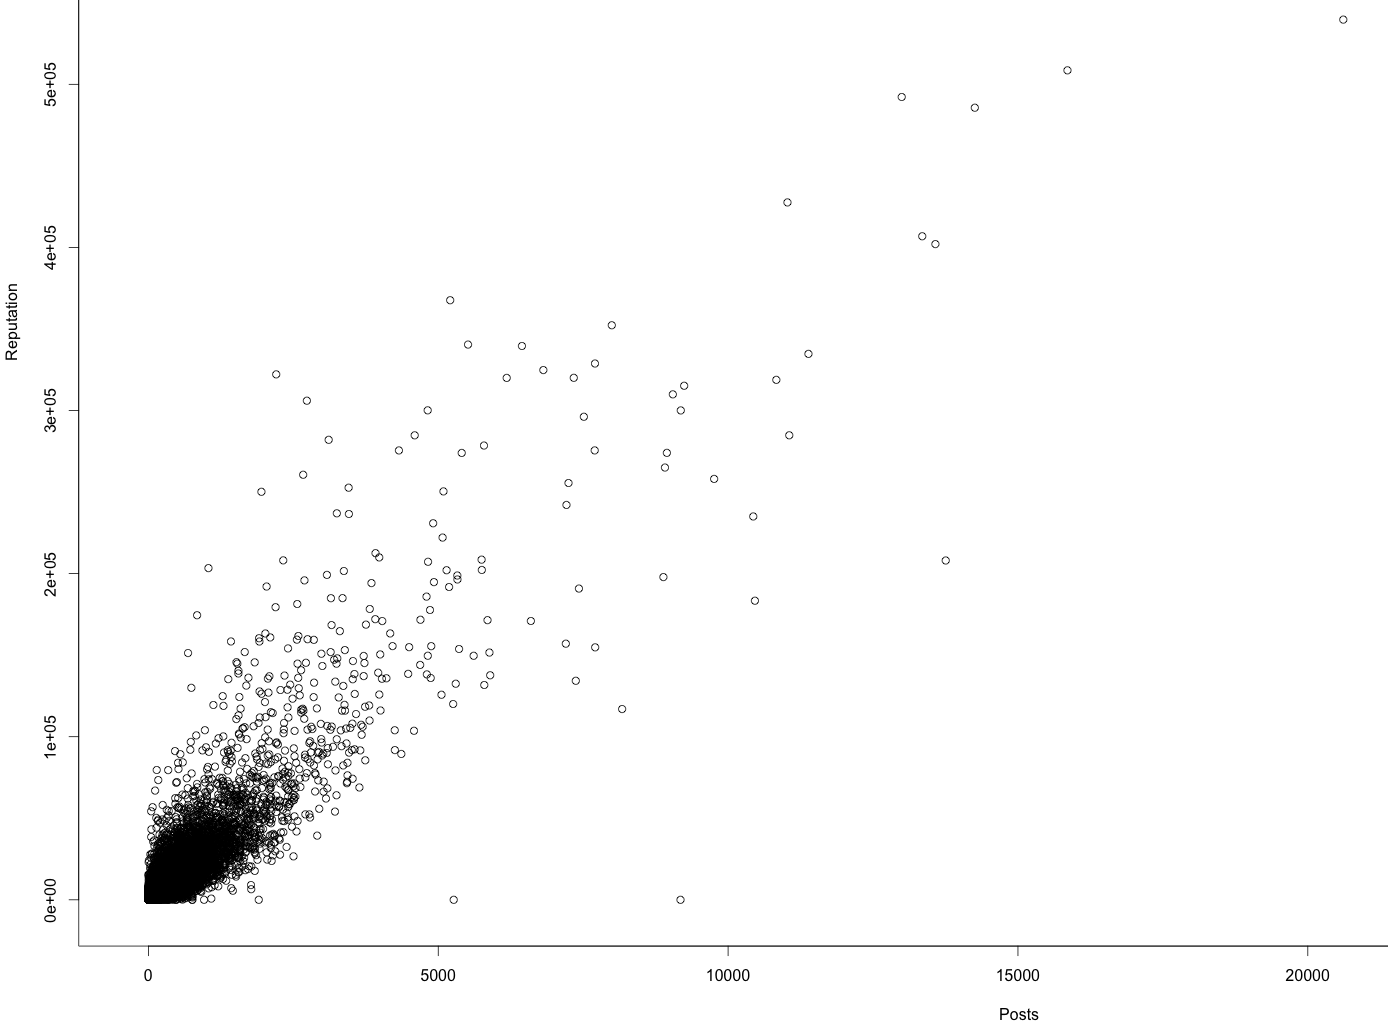
\includegraphics[width=9cm]{Plots/answers_vs_rep.png}
 \caption{The number of posts a user made compared to the reputation she gained}
 \label{answers_vs_rep}
\end{figure}

\begin{figure}[h]
 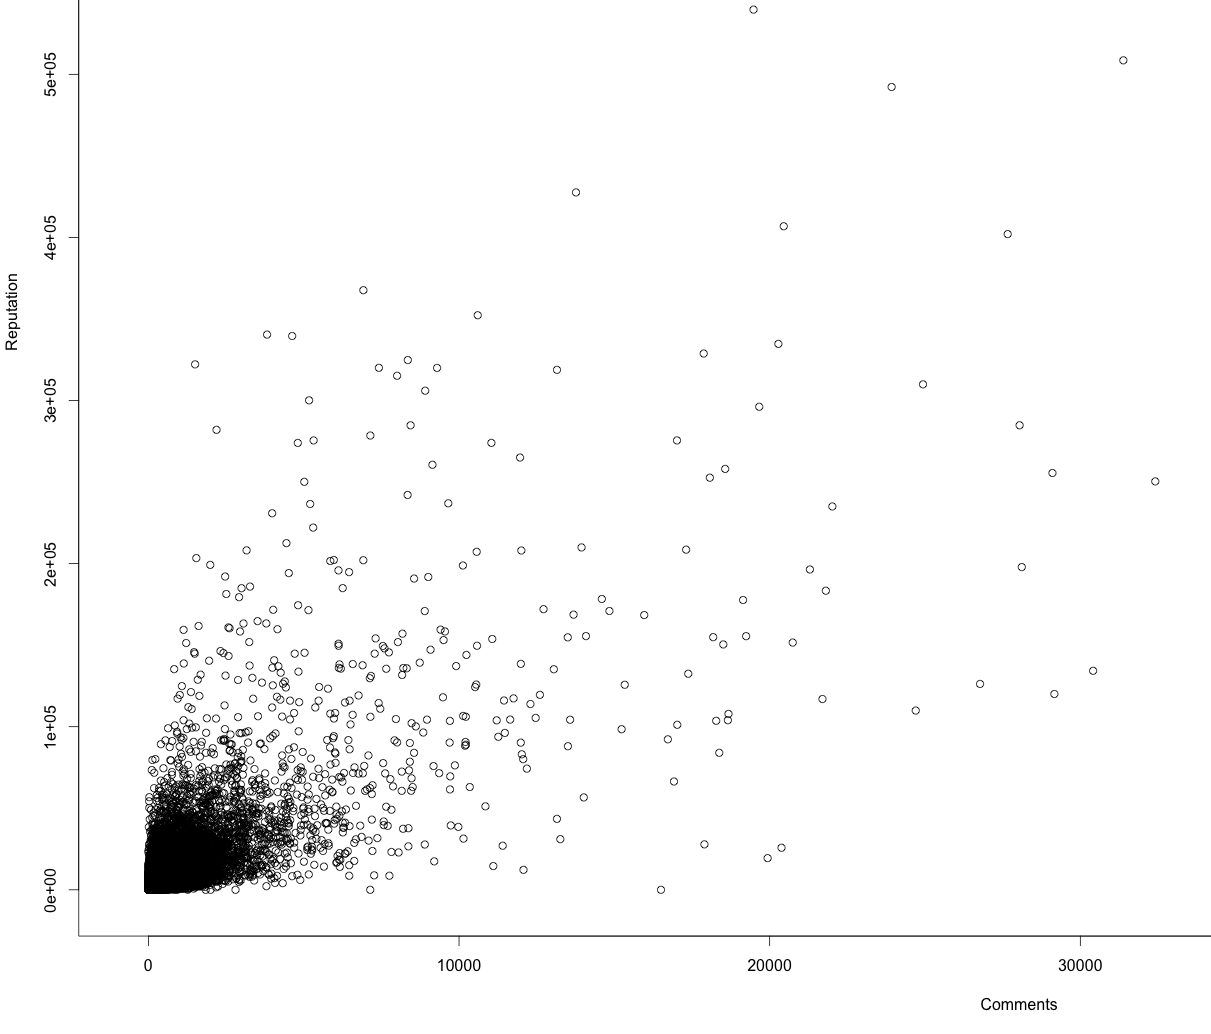
\includegraphics[width=9cm]{Plots/comments_vs_rep.png}
 \caption{The number of comments a user made compared to the reputation she gained}
 \label{comments_vs_rep}
\end{figure}

\begin{figure}[h]
 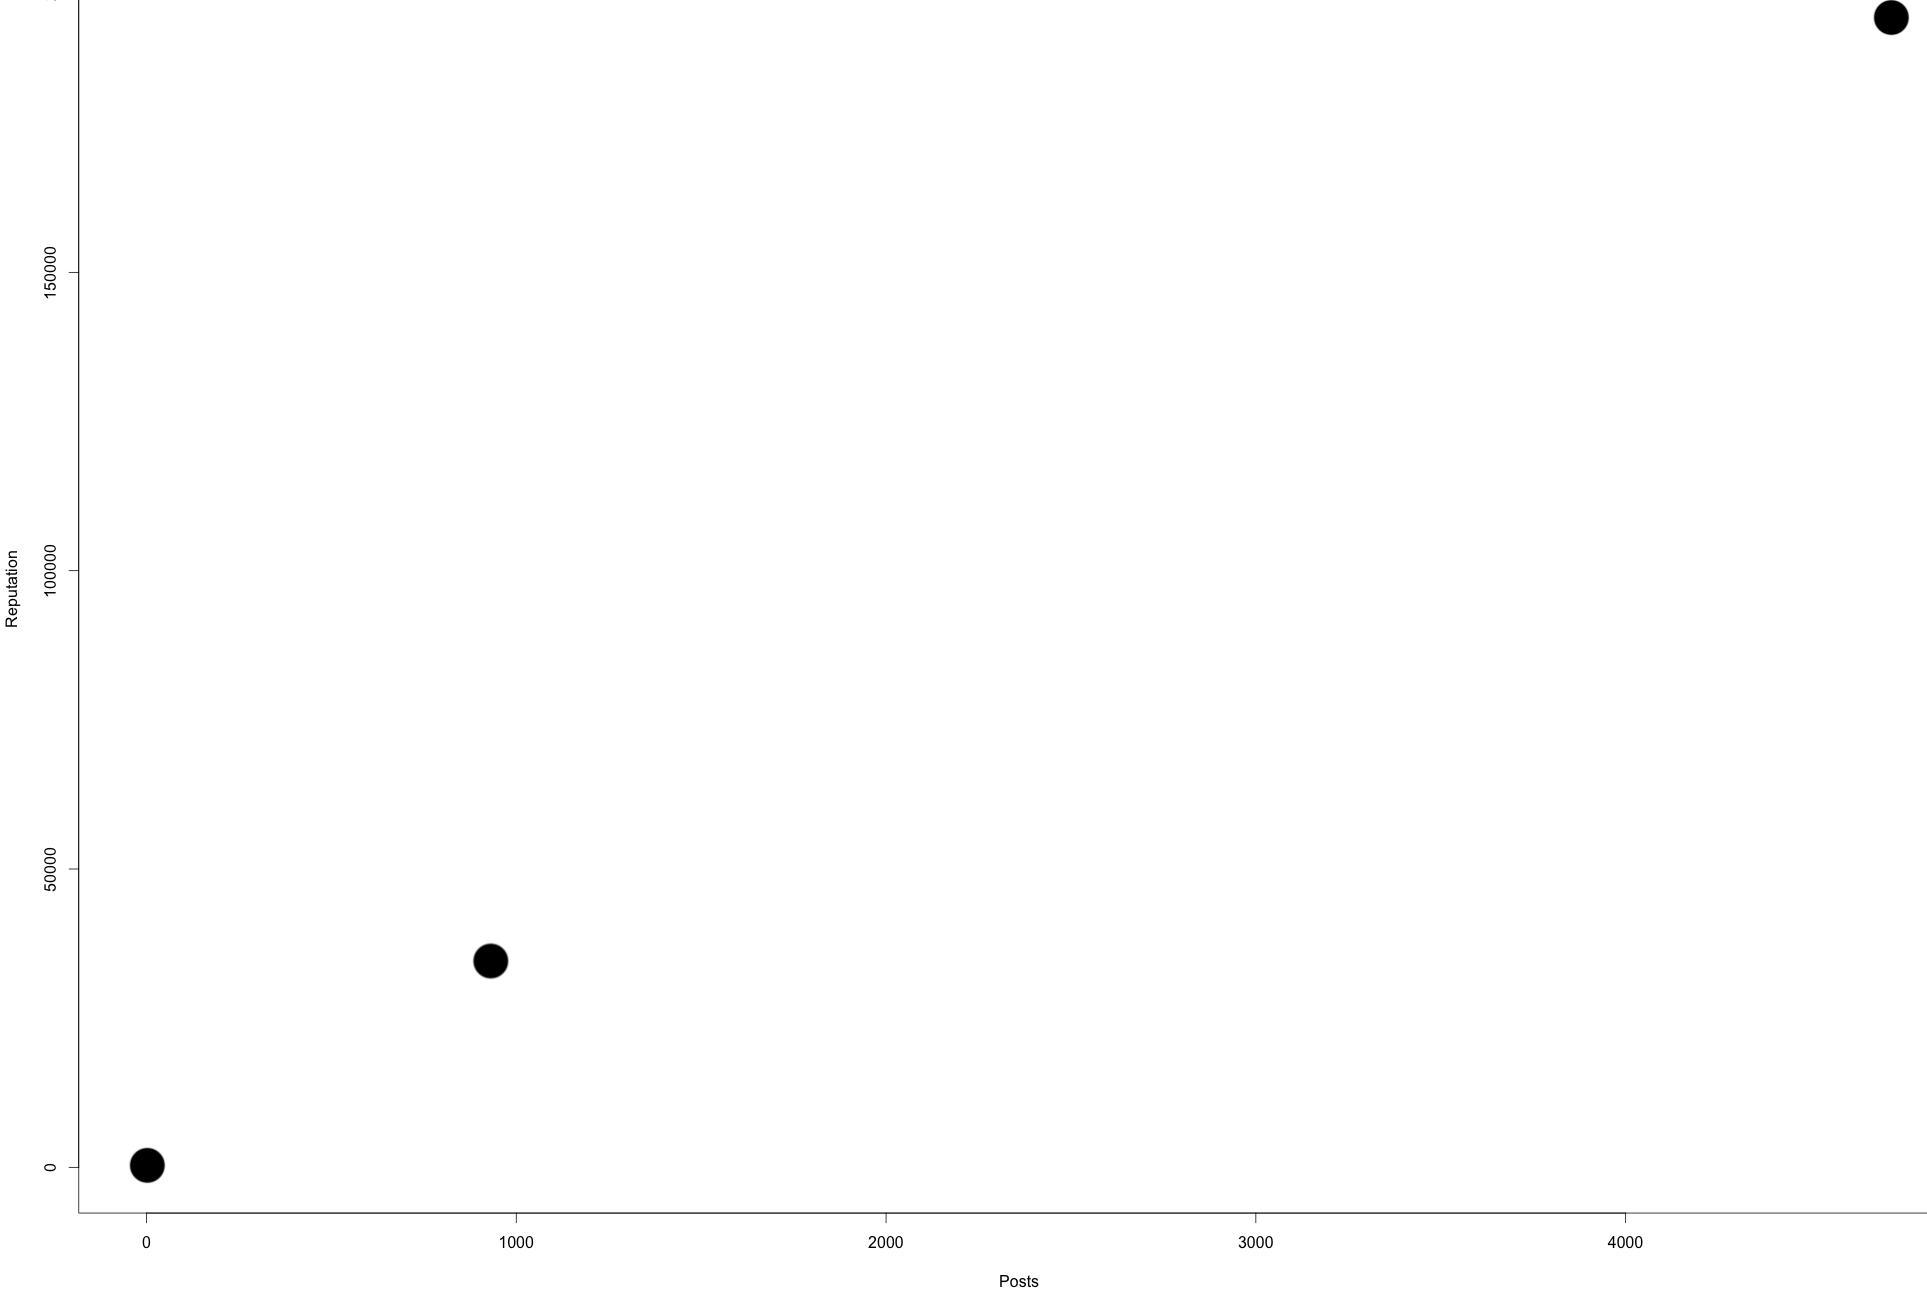
\includegraphics[width=9cm]{Plots/clustering.png}
 \caption{The clustering of the user groups}
 \label{kmeans_clustering}
\end{figure}


\section{Initial Assumptions}
\label{InitialAssumptions}

Before conducting the actual research, a number of assumptions was made. These assumptions formed the base for the research questions we try to answer.
\\
\\
One of the earliest assumptions, which is not tested, was that the group with largest number of users which are not active on the site at all, consists of so-called \textit{newbies}. These were more likely to not understand how the community of StackOverflow works, and may ask trivial questions which are not suitable for the level of expertise StackOverflow aims for.
\\
\\
% Assumption of duplicate questions
More testable assumptions were also made. Many users which would register on the website could, because of their unfamiliarity with the system, ask questions which had been asked previously. These questions are quickly flagged by the community as \textit{duplicate}. However this may be the appropriate action for the community as a whole, it can be extremely discouraging for the user which posted the question. Our research question is then: \textit{Are users which have posted only one question more likely to have created questions which are marked as duplicates}.
\\
\\
% Assumption of uncommon tags
It may also be the case that these users got discouraged due to some other reason, such as asking questions about uncommon topics. In case their question was regarding a topic with hardly any experts on the StackOverflow platform, the user again can get discouraged by the lack of comments or answers to guide them into the right direction. However, simply parsing the content of the question is not sufficient. In order to be found by possible experts, it is also required for users to use the correct tags for their question. Otherwise, the question might simply get lost in enormous question set of StackOverflow. This gives the following research question on this topic: \textit{Are users which have posted only one question more likely to have posted questions with uncommon tags}.
\\
\\
% Assumption of deletions
Another possible explanation for the large number of users with a low question count can also be found in deletions. Users themselves can delete questions after posting them, and so can the community's moderators. This can have quite an impact. As studied in \cite{correa2014chaff}, deleted questions usually are of a very low quality (the quality is considered low compared to the expectation of the StackOverflow community). Users unfamiliar with the ethos of StackOverflow may inadvertently post such questions, only later realizing these do not belong there, and be deleted (or be deleted by moderators). This gives rise to the following research question: \textit{Are users which have posted only one questions more likely to have their posts removed (either themselves or by a moderator / community)}.
\\
\\
% Assumption of less views
Additionally it may be the case the user question was not viewed as much as they had anticipated, resulting in fewer good answers. It may be the case their question was listed lower due to their lack of reputation, or simply got lost in the list of questions. Apart from that, it is also possible that questions from people with no post history simply get opened less often, resulting in lower quality answers. Since a low view count can also, to some extent, discourage the question askers, since he or she may feel neglected by the community. The research question following from the above yields the following: \textit{Are users which have posted only one question more likely to attract less views to the question he or she posted}.
\\
\\
% Assumption of unanswered questions
The final assumption that was made is that new users simply got let down by the community: they asked a question which did not violate any of the StackOverflow rules, but did not receive a (satisfactory) answer anyway. This would probably the most discouraging situation, since the user did not do anything wrong, but did not receive help due to aspects out of his or her control. That might cause them to lose the confidence in the community itself. This yields the following research question: \textit{Are users which have posted only one question more likely to have received no answer to their original question}. 

\section{Methodology}
\label{Methodology}

In this section we describe the methodology used to gain answers on our research questions which we specified in the section \ref{InitialAssumptions}.

\subsection{Processing the data}

The data used was made available by StackOverflow itself and also used for the 2014 MSRChallenge \cite{msrchallenge-website}. The export consisted of the (filtered) data of several key tables of the StackOverflow website. The data was formatted in XML files, which makes it hard to query directly on the data. This is why the decision was made to implement a multithreaded data loader which stored the XML data into a MSSQL database. Although the process took two days to complete, this proved to be worth the effort: it allowed to do large analysis on the entire data set instead of restricting the analysis to subsets.
\\
\\
For the actual querying, statistical analysis, and plotting of the data a mixture of Ruby, C\#, and R was used. Whereas Ruby was used for mining additional data,  both C\# and R showed their value in querying the data and performing statistical analysis. In the end R was used to generate any plots which were able to shed more light on the data.


\subsection{Evaluation of Duplicate questions}
In order to answer the research question \textit{Are users which have posted only one question more likely to have created questions which are marked as duplicates}, a comparison between percentage of duplicate questions  between all users and one-day flies should give similar results. Thus the methodology is to first find all users with only one question asked, then check whether the question is marked as duplicate (by checking on  LinkTypeId in the PostLinks table) and do the same for all questions in the StackOverflow data. This holds because the total amount of questions asked by one-day flies is less than $8\%$ of the complete question set. After retrieving these results a simple comparison should show whether one day flies post more duplicate questions in comparison to the complete user base.

\subsection{Evaluation of Uncommon tags}
%short recal of the assumption followed by a method to verify this assumption
In \cite{correa2014chaff} researchers were able to find over $3.300$ tags that only occur in questions of quality far below StackOverflow standards. The research question \textit{Are users which have posted only one question more likely to have posted questions with uncommon tags} is based on these findings, as similar results might be found. The methodology for answering of this research question is to look at top $50$ most popular tags given to one-day fly questions in comparison to the top $50$ tags given in all questions in Stack Overflow. This should give enough insight in the most popular tags and the existence of a popular uncommon topic among one-day flies.

\subsection{Evaluation of deletions}
%short recal of the assumption followed by a method to verify this assumption

The number of deletions is not directly obtainable from the database dump as provided by StackOverflow. Therefore two sample sets were taken, with a size of $150.000$; one for people with a low post count, and one for people with a high post count. For each of these sets, the corresponding StackOverflow page was fetched, and its DOM structure was parsed. This allowed to extract whether the question was deleted, or possibly closed.

\subsection{Evaluation of less views}
%short recal of the assumption followed by a method to verify this assumption
It might be possible that one-day flies simply have received less views on their posts.
In order to correctly determine this, data set was assembled with a distinction between one-day-flies and regular users. To examine the results, it might be useful to eliminate the highest viewed questions and the least viewed questions  from the data set. For this, we select the percentages of 5\%, 10\%, and 20\%. Based o the results with exclusion of these 5\%, 10\% and 20\% we can answer the research question \textit{Are which have posted only one question more likely to attract less views to the question he or she have posted}.\\


\subsection{Evaluation of unanswered questions}
%short recal of the assumption followed by a method to verify this assumption

As stated earlier, it may be possible for one-day-flies that their questions are simply not answered that often (especially compared to veteran community members). To model this, two sets were taken. The set containing the questions for the one-day-flies had a size of $1.016.696$, whereas the set containing the questions for the more active users consisted of $6.578.818$ questions.

\section{Results}

In this section we present the results of the evaluation of each research question as described in section \ref{Methodology}

\subsection{Duplicate questions}

The number of duplicate questions is surprisingly low. One could expect that this would be high on a public Q\&A community where a large percentage of the users is unfamiliar with platform. However, only $2.2\%$ of the one-day flies questions is marked as a duplicate. Meanwhile, this percentage increases to $2.9\%$ for the regular users. This would be surprising, since one can assume that regular users are more familiar with the platform and its search functionality. Based on this data we can say that the answer to the research question \textit{Are users which have posted only one question more likely to have created questions which are marked as duplicates} is no.

\subsection{Uncommon tags}

Surprisingly enough the top-5 tags of both one-day flies and regular users are identical (although ordered different). Although there are a number of tags which are specific to one-day flies, a large number of them is very similar.This allows us to answer the research question \textit{Are users which have posted only one question more likely to have posted questions with uncommon tags}. with no.

\subsection{Deleted questions}
As it turned out, the number of deleted questions for low post count users was $15.4\%$, whereas it was $10.9\%$ for the high post count users. However, it cannot easily be determined what the reason for deletion was. As explained in \cite{correa2014chaff}, there are several reasons for a question to be deleted. Without additional information, more research is needed to determine whether this can be a factor in the user participation. This research question therefore can not yet be answered.
\\
\\
The same analysis also gave interesting insights in the number of closed posts. For both groups, this turned out to be surprisingly low: $0.92\%$ for low post count users, and $0.76\%$ for high post count users. Questions can be closed for various reasons, such as being a duplicate or for being off-topic. Closed questions may be improved or deleted later on. However, the difference between the number is quite low , which allows us to answer the research question \textit{Do one-day flies more often have their questions removed?} with no.

\subsection{View counts}
As it turns out, both groups have an average view count of around $190$ (for one-day-flies this was $198$, for regular users $187$). However, the view count cannot be used only to determine this, since the standard deviation for these groups was quite high (respectively $400$ for one-day-flies, but over $1.000$ for regular users). To compensate for these effects, the dataset was modified to only include the posts which fitted into the $10\%$ to $90\%$ range of the view counts, and the results were rerun.
\\
\\
Using this reduced data set, with the extremes removed, a similar result is obtained, with an average view count of $127$ for one-day-flies and $113$ for non-one-day-flies. The standard deviations dropped a lot as well, to only $100$ respectively $93$. When the analysis is repeated by eliminating the extreme $5\%$ of $20\%$, similar results remain.
\\
\\
Therefore we conclude that the posts of one-day-flies are actually not viewed less than those of non-one-day-flies, since it any case the view count of the latter group is actually lower. The research question \textit{Are users which have posted only one question more likely to attract less views to the question he or she have posted} is therefore no.

\subsection{Unanswered questions}

Based on the data there seems to a difference between the two user groups. The group of one-day-flies has a larger percentage of unanswered questions: $17\%$ compared to just $10\%$ for the group which has a higher post count. Here we see a  difference between the two groups. It might very well be the case user get demotivated because of this, especially if they saw other users receive answers to their posts much more often. Since this difference on the complete dataset is only 7\% we can answer the question \textit{Are users which have posted only one question more likely to have received no answer to their original question} with yes, but can argue that this is only a very slight difference, thus does not indicate the reason why one becomes a one-day fly.


\section{Qualitative research}\label{QualitativeResearch}
Since the results did not reveal a clear reason which explained the existence of one-day flies, we decided upon a small qualitative research to get new ideas and see if something was overlooked that can be found in the data itself rather easily.  For this the authors manually scanned through $50$ posts and their accepted answer, answering the following questions:

\begin{enumerate}
\item Does the question contain code?
\item Does the accepted answer contain code?
\item Does the question contain a clear explanation?
\item Was the answerer friendly or unfriendly in his answer?
\item Did the question asker put in enough effort (was the answer not easily found by using any search engine)?
\end{enumerate}

After answering these questions the results for the sample where as follows:
\newline
\newline
\begin{tabular}{ | l | p{8cm} | }
\hline
  1 & $20$ questions contained code \\
\hline
  2 & $19$ accepted answers contained code \\
\hline
  3 & All the $50$ questions contained an explanation \\
\hline
  4 & $48$ answerers where friendly, $2$ where unfriendly \\
\hline
  5 & $11$ times the answer was easily found by a search engine, the other $39$ times they tried to find a solution themselves \\
\hline
\end{tabular}
\newline
\newline

The results of 1 and 2 show that over half the questions and accepted answers did not contain code, even though the questions where programming related. Most of them where regarding versioning systems, or development methods (such as Agile or database systems).  However it still might be interesting to look at the code example quality as this seemed relatively poor in the sample the authors took.
\\
\\
The result of 3 is not a surprise, however the results of 4 is interesting. Two answers where unfriendly, but still got accepted. This gives the idea for a new research question: Do one-day flies  not come back due to negative feedback? 
\\
\\
The result of 5  gives the idea that askers are relatively ``lazy''. However, since the classification ``lazy'' is quite opinionated, this cannot be used as a direct research result. However the authors did find during this qualitative research was that a few questions where later answered by the question owner him/herself. This gave the idea that one-day flies might only use StackOverflow for self-documentation purposes. 
\\
\\
To get a better insight in questions 1, 2 and 4: we did an automated search for this. For question 1 and 2 this was easily done using R. For question 4, a Ruby script with SentiStrength \cite{sentistrength} was used to evaluate how friendly the answers and questions were on a scale of -4 (very unfriendly) to 4 (very friendly). 
\\
\\
For question 1, it turned out that for non one-day flies $65\%$ of the questions had code, and $58\%$ of the answers (over the set of all questions with an accepted answer). For one-day flies these numbers were $70\%$ and $65\%$ respectively. This indicates one day flies give and receive a bit more code than the other users.
\\
\\
To answer the friendliness, a random subset of $10000$ questions with an accepted answer was taken. It turned out that non one-day-flies questions had a niceness of $0.079$, and the answers they received had a niceness of $0.059$. This indicates that both the questions and answers were mostly formal and professional, and on average slightly positive.
\\
Again this was a bit different for one-day flies: they had a question niceness of $0.196$ and received an answer with niceness $0.092$. Still the tone appears to be mostly formal and professional, but the underlying touch tends to be a bit more positive.

\section{New Research Questions}
\label{NewResearchQuestions}

Based on the work presented in the previous chapter, the authors formulated a number of new research questions. This might form the basis for future work regarding the participation of \textit{one-day-flies} on Q\&A communities such as StackOverflow.

%Assumption of bad code examples
\subsection{Code example quality}

In general it seems the quality of the code examples in questions of one-day-flies is lower compared to the quality of users with a higher reputation. One-day-flies generally include too much code (by simply pasting all the code into the questions code block. This discourages users to form an adequate explanation.
\\
\\
Apart from that, the general code quality itself is lower as well. Code is poorly modularized, which causes people to respond to those issues, before addressing the original problem of the question asker. He or she may then get irritated, since they receive feedback they simply are not ready for at that point in the learning process. The same goes for the people trying to figure out what the issue is: they need to wrap their mind around to some non-standard principles used by others, which are (from their perspective) less easy to reason about.

%Assumption of negative feedback from the community
\subsection{Negative feedback}

As stated in the previous paragraph, it is often the case the StackOverflow community gives tips and advice to novices how certain problems should be structured. However, for the question asker this can be seen as negative feedback. It does not solve their problem, while it increases the work they have to do in order to solve the problem or even get community support.
\\
\\
Even without this feedback, the StackOverflow community has strict rules on the type of questions allowed on the platform. A quick search over time showed the authors that these rules were not strictly followed in the early days of the StackExchange platform, but are more followed these days. This causes many beginners questions, subjective discussions (\textit{Is A better than B?}), or too-localized questions (\textit{What does this regular expression do?}) to be voted for closing or deletion.
\\
\\
Since the community has answered a large number of questions, one can expect the same thing to happen for other things, such as \textit{marked as duplicate}. The chances are increasing that somewhere in the database, a very similar question might have been asked already, and received an appropriate answer. Meanwhile, a beginner on the platform might not be aware of the exact terminology to find that specific question. Therefore they may consider their problem to be new and unique, causing them to post it. Several minutes later, they may find their question marked as a duplicate combined with a snide comment on "how you can search on StackOverflow". Little imagination is needed to see how a user would see this as a negative feedback from the community.


%This section is written after writing the qualitative research section thus doesn't have to be revised (only spell/grammar checked)
\subsection{Self-answering}
In section \ref{QualitativeResearch}  the authors found that some of the questions accepted answers where given by the authors of these questions. This could be done for documentation purposes, but also for attempting to gain reputation, while other answers might be better. However in order to explore this further, it is first interesting to evaluate whether one-day flies more often answer their own questions than non-one-day flies on StackOverflow.
\\
\\
A user does not get reputation for answering their own question (but they can get reputation if the answer is upvoted by others). Here there seems to be a clear trend: users have found and answer, and decided to share it with the community (even though they do not have a direct profit from it themselves). This seems to be an indication these users are not scared away from StackOverflow at that point (otherwise they likely would not have posted that answer). 

\subsection{Everything can be found}
During the research the authors had several discussions with other developers regarding this high amount of one-day flies. In most of these sessions developers said to never ask a question on StackOverflow because the answer to their question is already available. This gave the authors a new idea that possibly almost all questions can be found, thus the chance that a user has two questions that are not answered on StackOverflow already is rather slim. This could cause the community to look like it has many one-day flies whereas the one-day flies just have one question that could not be found on StackOverflow before. If this is the case, then when taking into account the user growth, one should see a decrease in the amount of questions asked over time. 

\section{Conclusion and future work}

As indicated by the previous sections, there does not seem to be a clear reason within these statistics why the group of \textit{one day flies} does contribute more to the platform. It therefore seems there are other reasons for one-day flies to stop contributing to the StackOverflow platform. In this paper, no definite conclusion can be given of the \textit{why} the vast majority of StackOverflow only posts one question. However a number of research questions were evaluated with their statistics shown in figure \ref{finalResults} , and more possible open research questions which can be found in \ref{NewResearchQuestions}, allowing for future work.

\begin{figure}[h]
 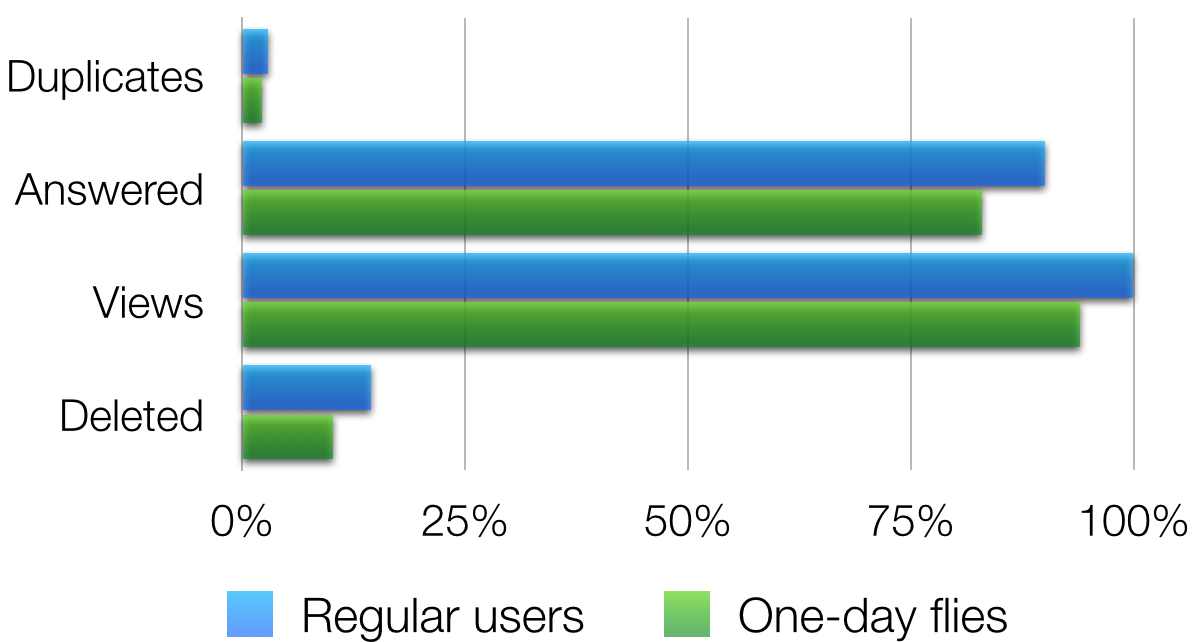
\includegraphics[width=9cm]{Plots/BarPlot.png}
 \caption{Results of the analysis}
 \label{finalResults}
\end{figure}



\begin{thebibliography}{1}

% MLA style

\bibitem{SOPopularity}
Anderson, Ashton, et al.
\emph{Discovering value from community activity on focused question answering sites: a case study of stack overflow.},
\hskip 1em plus 0.5em minus 0.4em\relax
Proceedings of the 18th ACM SIGKDD international conference on Knowledge discovery and data mining. ACM, 2012.

\bibitem{SOResearch1}
Treude, Christoph, Ohad Barzilay, and Margaret-Anne Storey.
\emph{How do programmers ask and answer questions on the web?},
\hskip 1em plus 0.5em minus 0.4em\relax
Nier track." Software Engineering (ICSE), 2011 33rd International Conference on. IEEE, 2011.

\bibitem{SOResearch2}
Barua, Anton, Stephen W. Thomas, and Ahmed E. Hassan.
\emph{What are developers talking about? an analysis of topics and trends in stack overflow.},
\hskip 1em plus 0.5em minus 0.4em\relax
Empirical Software Engineering 19.3 (2014): 619-654.

\bibitem{SOResearch3}
Morrison, Patrick, and Emerson Murphy-Hill.
\emph{Is programming knowledge related to age? an exploration of stack overflow.},
\hskip 1em plus 0.5em minus 0.4em\relax
Mining Software Repositories (MSR), 2013 10th IEEE Working Conference on. IEEE, 2013.

\bibitem{buildingrep}
Bosu, Amiangshu, et al.
\emph{Building reputation in stackoverflow: an empirical investigation.},
\hskip 1em plus 0.5em minus 0.4em\relax
Proceedings of the 10th Working Conference on Mining Software Repositories. IEEE Press, 2013.

\bibitem{repsystem}
Movshovitz-Attias, Dana, et al.
\emph{Analysis of the reputation system and user contributions on a question answering website: StackOverflow.},
\hskip 1em plus 0.5em minus 0.4em\relax
Proceedings of the 2013 IEEE/ACM International Conference on Advances in Social Networks Analysis and Mining. ACM, 2013.

\bibitem{correa2014chaff}
Correa, Denzil, and Ashish Sureka.
\emph{Chaff from the wheat: characterization and modeling of deleted questions on stack overflow.},
\hskip 1em plus 0.5em minus 0.4em\relax
Proceedings of the 23rd international conference on World wide web. International World Wide Web Conferences Steering Committee, 2014.

\bibitem{PersonalityTraits}
Blerina Bazelli, Abram Hindle, and Eleni Stroulia
\emph{On the Personality Traits of StackOverflow Users},
\hskip 1em plus 0.5em minus 0.4em\relax
2013 IEEE International Conference on Software Maintenance

\bibitem{sparrowsandowls}
Jie Yang, Ke Tao, Alessandro Bozzon, and Geert-Jan Houben
\emph{Sparrows and Owls: Characterisation of Expert Behaviour in StackOverflow},
\hskip 1em plus 0.5em minus 0.4em\relax
22nd International Conference, UMAP 2014, Aalborg, Denmark, July 7-11, 2014. Proceedings

\bibitem{msrchallenge-website}
A. Ying, et al.
\emph{Mining Challenge - MSR 2015},
\hskip 1em plus 0.5em minus 0.4em\relax
http://2015.msrconf.org/challenge.php

\bibitem{sentistrength}
Nielsen, Finn Årup.
\emph{A new ANEW: Evaluation of a word list for sentiment analysis in microblogs.}
\hskip 1em plus 0.5em minus 0.4em\relax
arXiv preprint arXiv:1103.2903 (2011).

\end{thebibliography}

% that's all folks
\end{document}